\section{What are fractals?}\label{what-are-fractals}

Fractals are objects with self-similarity, where the smaller fragments
are similar to those on a larger scale. A characteristic feature is to
have subtle details even at very high magnification.

\subsection{Mandelbrot set}\label{mandelbrot-set}

This is a typical example of a two-dimensional fractal generated
mathematically. This image is created with a very simple formula, which
is calculated in many iterations:

\[z_{n + 1} = z_{n}^{2} + c\]

``z'' is a complex number (\emph{a} + i\emph{b}), where i = (imaginary
number). The number is made of two parts : ``\emph{a}'' the real part
and ``i\emph{b}'' the imaginary part.

``c'' is the coordinates of the image point to be iterated.

In 2D, ``z'' is a vector containing two complex number coordinates , x
and y, ( these points represent the pixel location where x represents
the real part of the number {[}a{]} and y represents the imaginary part
of the number {[}b{]}). Because they are complex numbers, they can be
positive or negative, but also there will still be a mathematical
solution if a function requires the square root of a negative number.

Each original point (pixel position) is tested in the formula iteration
loop, to determine if it belongs to the formula specific mathematical
fractal set.

The initial value of point ``z'' is assigned to equal ``c'', (z0 = c),
this parameter is then used repeatedly in the iteration loop.

\(z_{n + 1} = z_{n}^{2} + c\)-iteration-\textgreater{}\(z_{n + 2} = z_{n + 1}^{2} + c\)-iteration-\textgreater{}\(z_{n + 3} = z_{n + 4}^{2} + c\)etc.

Termination conditions are applied to ensure the formula does not
iterate to infinity. The most common conditions used are called Bailout
and Maxiter. Maxiter is simply a condition to stop iterating when a
maximum numbers of iterations is reached.

The Bailout condition stops the iteration loop if the formula transforms
(moves) the point further than a set distance away from an ``origin''.

In the Mandelbrot formula, after each iteration, the modulus of a
complex number is calculated; in other words, the length of the vector
from the origin (x = 0, y = 0) to the current ``z'' point. This vector
length is often called ``r'' for it is the radius from the center
(origin) to the current ``z'' point.

In this example, when the length r \textgreater{} 2 (i.e Bailout = 2),
the termination condition has been met, then the iteration process is
stopped and the resulting image point is marked with a light color.
When, after many repeated iterations, ``r'' is still less than 2, then
it can be considered for simplicity that such a result will continue
indefinitely. Iterations are therefore interrupted after a certain
number of iterations (Maxiter). This point is marked on the image with
black. This results in a ``set'' of points that do not reach bailout
termination (black) and the rest of the points given lighter colors
(dependent on a chosen coloring method).

\subsection{3D fractals}\label{d-fractals}

The three dimensional fractal type, the "Mandelbulb," is calculated from
a fairly similar pattern to the Mandelbrot set. The difference is that
the vector ``z'' contains three complex numbers ( x, y, z) or four
dimensions (x, y, z, w). As they are part of the ``z'' vector, they are
denoted as (z.x, z.y, z.z). Examples being Hypercomplex numbers and
quaternions.

They can also be created by modification of quaternions or by a specific
representation of trigonometric vectors. Generally, common maths
operators are used, e.g., addition, multiplication, squaring, and
powers), and also conditional functions ( e.g., if z.x \textgreater{}
z.y, then z.x = something).

Some other types of 3D fractal objects are based on iterative algorithms
(IFS - Iterated Function Systems). An example would be the famous Menger
Sponge.

\subsection{Mandelbulber Program}\label{mandelbulber-program}

Mandelbulber is an easy to use, handy application designed to help you
render 3D Mandelbrot fractals called Mandelbulb and some other kind of
3D fractals like Mandelbox, Bulbbox, Juliabulb, Menger Sponge, \ldots{}.
The following sections cover the program interface and give useful
information about how to use it.

\section{Distance Estimation}\label{distance-estimation}

Distance Estimation (DE) is the calculation of an estimated distance
from the given point to the nearest surface of the fractal. As suggested
by the word 'estimate', it is an approximate value. It is calculated
using simplified algorithms based on analytical (Analytical DE) or
numerical (Delta DE) calculations of gradients.

DE is the most important algorithm required to render three-dimensional
fractals within a reasonable time. It achieves a great reduction in the
number of steps needed to find the exact area of the fractal while
tracking a ``photon'' traveling toward the object along a ray (a
simulated beam of light from the camera eye). A ray is generated for
each pixel (1000 x 1000 resolution = 1,000,000 rays). They match FOV
from the camera eye (i.e. they are not parallel.)

Without the DE calculation, the proximity of the photon to the fractal
surface would need to be repeatedly calculated after each of many very
small steps. For example, without an estimate of where the fractal
surface is, you may need up to 10,000 steps to trace a ray of light, for
every pixel of the image.

Using DE, the size of the steps along the ray of light can be increased,
based on the calculated estimate of where the fractal surface should
approximately be located. The process of moving along the ray and
testing for the surface location is called ray-marching.

Ray marching looks like the illustration below. In each step, an
estimation on the distance to the nearest fractal surface is calculated.
The photon is moved along the ray by this distance. The next step is
re-calculated based on the estimated distance. This distance is less so
this time the Photon is moved a smaller distance. The ray-marching
becomes more accurate closer to the surface of the fractal. The ray
marching ceases when the photon becomes within a set ``distance
threshold'' from the surface or after a maximum number of iteration if
the option ``stop at maximum iteration'' is enabled.

Since the estimation contains some error (sometimes quite large), there
is a risk that the step of moving the "photon" will be too large, and
incorrectly it will flow into the surface of the fractal. This may
result in visible noise in the rendered image.

To prevent this, the "photon" can be moved by the estimated distance
multiplied by a number between 0 and 1 ("ray-marching step multiplier").
Steps are then smaller, so there is less risk of "overshooting" the
surface, but the rendering time increases due to more steps being
required.

Below is an example for a step multiplier of 0.5:

Each formula is assigned a DE mode and function (``preferred''). In most
cases the preferred \emph{mode} is Analytical DE (fastest).

The preferred \emph{function} is assigned based on whether the formula
is transforming in a linear or logarithmic manner. These setting can be
varied on the Render Engine tab.

Analytical DE mode is faster than Delta DE mode to calculate. However
with some formulas only Delta DE mode will produce a good quality image.
The DE modes can be used with either linear or logarithmic DE functions.

Example linear out-\textgreater{}distance = r / fabs(DE);

Example logarithmic: out-\textgreater{}distance = 0.5 * r * log(r) / DE;

The quality produced by the DE mode and function combinations is formula
specific. The setting of formula parameters can also greatly affect the
quality produced by the DE. In some cases the choice of fractal image is
determined by what location and parameters can produce good DE quality.

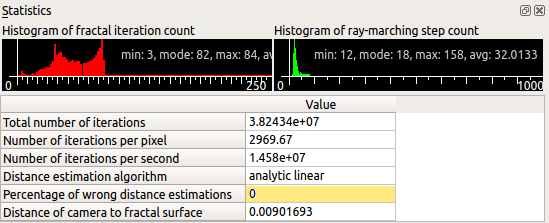
\includegraphics[width=5.71890in,height=2.32283in]{img/manual/media/image6.png}

In the Statistics (enable in View menu) you can see Percentage of Wrong
Distance Estimations ("Bad DE"). As a general rule less than 0.01 is
good, but it is case specific and 3.0 sometimes is OK and 0.0001
sometimes is not.

\section{Ray-marching - Maximum number of iterations vs. distance
threshold
condition}\label{ray-marching---maximum-number-of-iterations-vs.-distance-threshold-condition}

The \emph{ray marching distance threshold} is the condition where the
photon marching along the ray comes within a specified distance from the
fractal surface and the ray-marching stops. This controls the size of
the detail in the image, and is normally set to vary such that greater
detail is obtained for the surface closest to the camera, (in the
further regions of the fractal the distance threshold will be larger
such that only bigger details are visible). Enabling ``Constant Detail
Size'' on the Rendering Engine tab will make the distance threshold
uniform.

There are two modes of stopping the ray-marching of each image pixel.

1st case: Stop ray-marching at distance threshold (``Stop at maximum
iteration'' is disabled).

\protect\hypertarget{__DdeLink__1111_813559202}{}{}2nd case: Stop
ray-marching at point when a maximum number of iterations is reached
(``Stop at maximum iteration'' is enabled).

First important note: ``Stop at maximum iteration'' doesn't control the
fractal iteration loop. The iteration loop always runs to achieve
Bailout, (then if bailout is not reached the iteration stops at
Maxiter.).

\begin{longtable}[]{@{}ll@{}}
\toprule
\textbf{Example for 1st case:}

Ray-marching stops at distance threshold. In most cases the fractal
iteration loop stops on bailout condition, (because away from surface it
is not possible to reach Maxiter). & \textbf{Example for 2nd case:}

Ray-marching stops at the photon step when the maximum number of
iterations is reached (ray-marching distance threshold is ignored). In
many cases iteration loop stops on bailout condition (away from fractal
surface), but on the fractal surface the maximum number of iterations is
calculated (when bailout is not reached).\tabularnewline
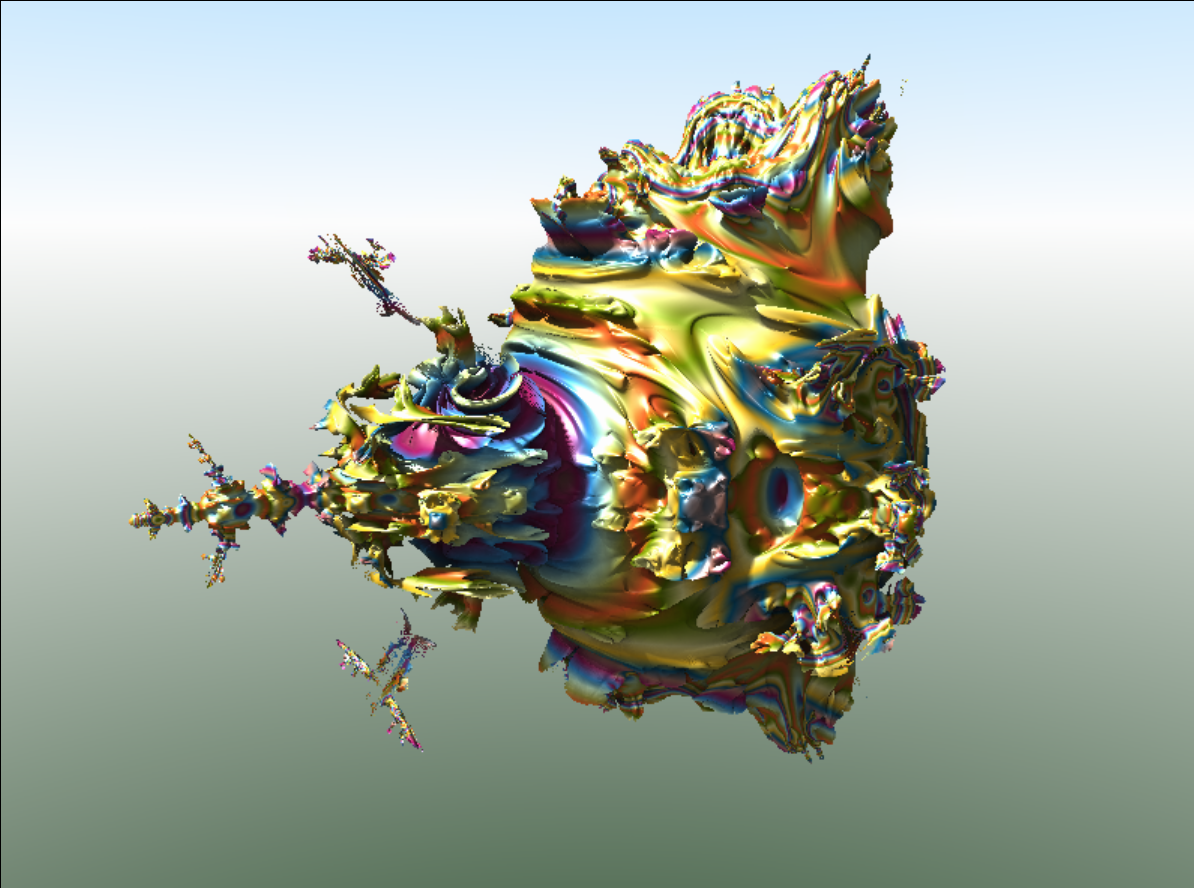
\includegraphics[width=3.22795in,height=2.40000in]{img/manual/media/image7.png}
&
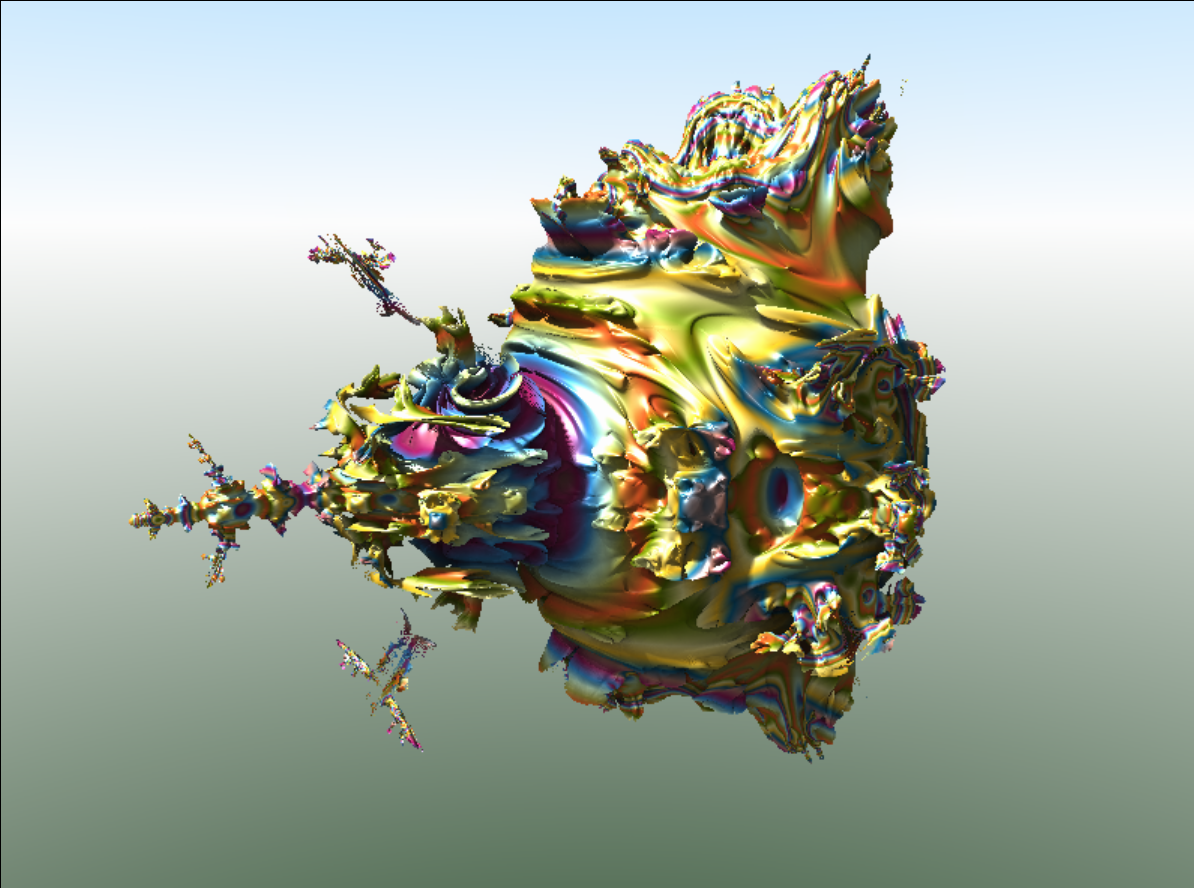
\includegraphics[width=3.26890in,height=2.44016in]{img/manual/media/image8.png}\tabularnewline
\bottomrule
\end{longtable}

\begin{longtable}[]{@{}ll@{}}
\toprule
\textbf{Example for 1st case:}

When maximum number of iterations is set to 4. Even if Maxiter is
reached the ray-marching is continued until the ray marching distance
threshold is reached. & \textbf{Example for 2nd case:}

When maximum number of iterations is reached, then ray-marching is
stopped even if distance threshold is not reached.\tabularnewline
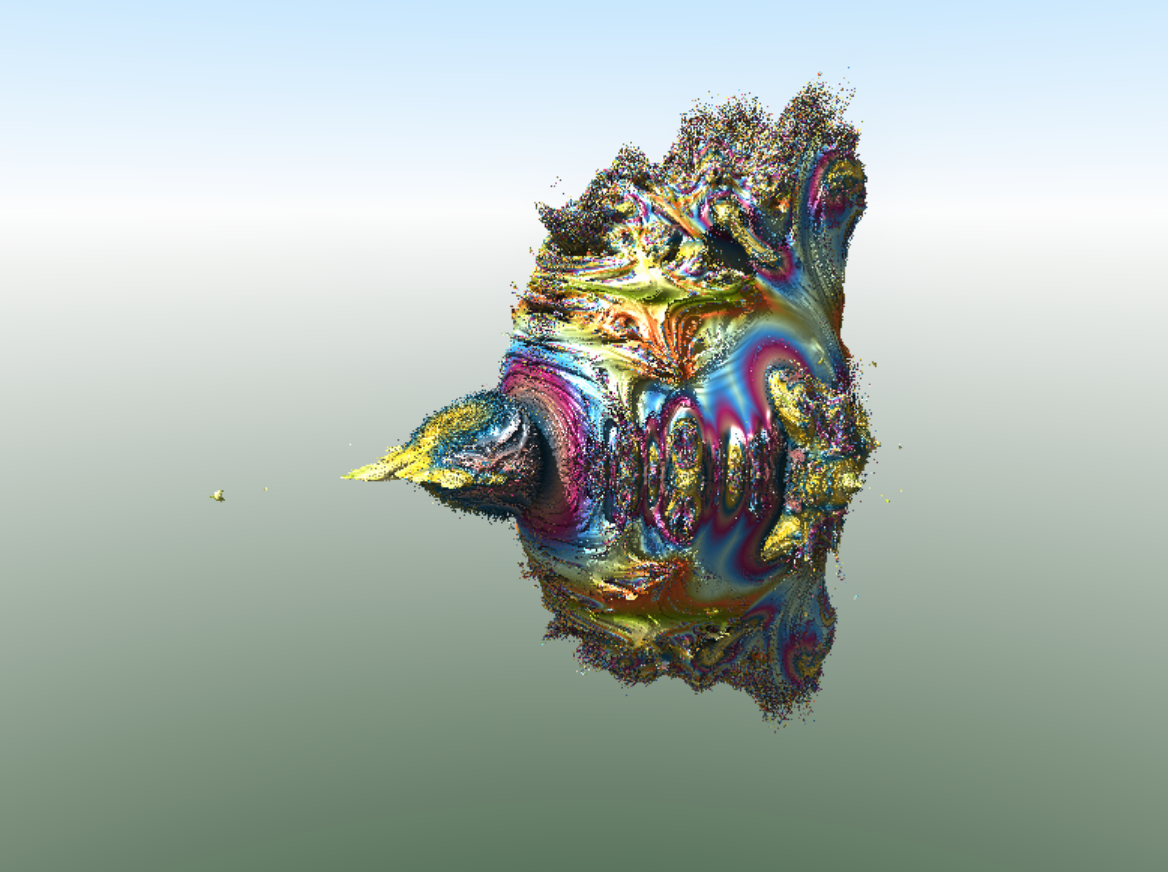
\includegraphics[width=3.26929in,height=2.44016in]{img/manual/media/image9.png}
&
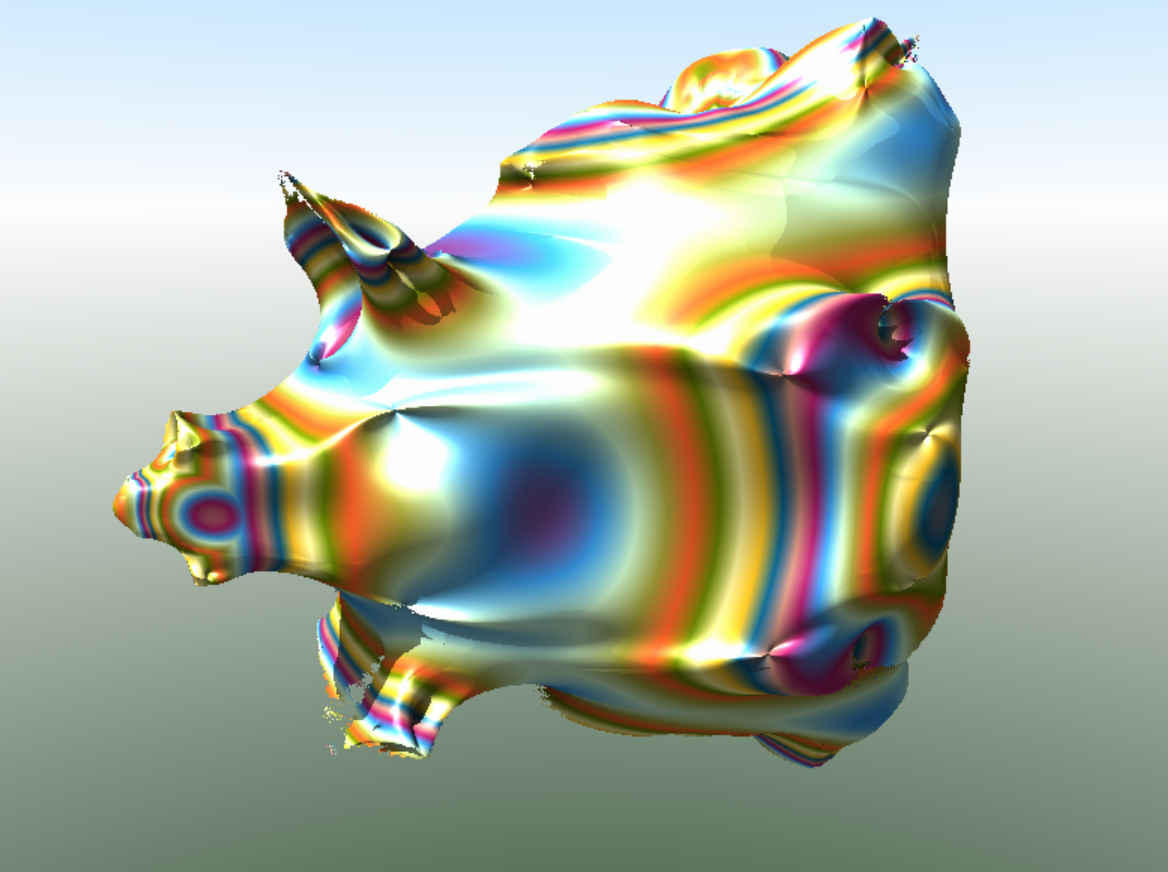
\includegraphics[width=3.26890in,height=2.44016in]{img/manual/media/image10.png}\tabularnewline
\bottomrule
\end{longtable}

\section{Navigation}\label{navigation}

To set the current view there are two elements:

\begin{itemize}
\item
  \textbf{Camera} - represents a point where the camera is located
\end{itemize}

\begin{itemize}
\item
  \textbf{Target} - represents the point to which the camera is
  orientated with (i.e., the camera is \emph{always} looking at the
  target.)

  \begin{enumerate}
  \def\labelenumi{\arabic{enumi}.}
  \item ~
    \subsection{Camera and Target movement
    step}\label{camera-and-target-movement-step}
  \end{enumerate}
\end{itemize}

The relationship between the camera point and the target point can be
altered manually by changing the numbers in the spin boxes, or by
navigating with distance and rotation ``steps'' defined by the user.

For rotations, the camera is moved by the parameter \textbf{rotation
step} (default 15 degrees). For movements of the camera and/or the
target in a linear direction, the parameter \textbf{step} (default 0.5)
is used. There are two modes for its use:

\subsubsection{Relative step mode}\label{relative-step-mode}

The \textbf{step} for moving the camera and/or target in a linear
direction is calculated relative to the estimated distance from the
surface of the fractal. The closer to the surface that the camera is
located, the smaller the step. This prevents movement of the camera
beneath the surface of fractal, because very close to the surface, a
step needs to be very small.

The actual step is equal to the distance from the fractal multiplied by
the parameter \textbf{step}.

Example: If in this mode, the step is set at 0.5 and the nearest point
of the fractal is 3.0, this camera will be moved 1.5 (no matter in which
direction).

This mode is recommended in animations approaching the surface of the
fractal.

\subsubsection{Absolute step mode}\label{absolute-step-mode}

Step movement of the camera and/or target is fixed. Therefore if the
step is set at 0.5, the movement will be 0.5 in the direction of the
arrow key or mouse pointer.

This mode is recommended for animation camera flying with a fixed (or
strictly controlled) speed.

\begin{enumerate}
\def\labelenumi{\arabic{enumi}.}
\item ~
  \subsection{The camera and target
  functions}\label{the-camera-and-target-functions}
\item ~
  \subsection{Linear camera and target movement modes using the arrow
  buttons}\label{linear-camera-and-target-movement-modes-using-the-arrow-buttons}
\end{enumerate}

A user can navigate by operating the arrow keys on the Navigation dock,
with the user defined steps.

There are three modes for changing the relationship between camera and
target.

\subsubsection{Move camera and target
mode}\label{move-camera-and-target-mode}

Moves both the camera and the target by the same distance in the same
direction. The angle of camera rotation does not change.

\subsubsection{Move camera mode}\label{move-camera-mode}

Moves only the camera and rotates it in respect to the motionless
target.

\subsubsection{Move target mode}\label{move-target-mode}

Moves only the target while maintaining a fixed camera position. The
camera rotates following the target. \textbf{Note:} In Relative Step
Mode, the target is moved by distance related to distance of target to
fractal surface. If target is inside the fractal (distance = 0), then
this option will not work with Relative Step Mode.

\subsection{Linear camera and target movement modes using the mouse
pointer}\label{linear-camera-and-target-movement-modes-using-the-mouse-pointer}

A user can navigate in the render window with the user-defined
\textbf{step} (absolute or relative) and the Mouse Click Function set to
``Move the camera.''

\subsubsection{Move camera and target
mode}\label{move-camera-and-target-mode-1}

The target is moved to the point selected by the mouse. The camera is
moved by a user defined step, and rotated.

In relative step mode, the camera is moved by distance equals to
\emph{distance\_to\_indicated\_point} multiplied by \emph{step}
parameter\emph{.}

In absolute step mode, the camera is moved by distance equals to
\emph{step} parameter\emph{.}

\subsubsection{Move camera mode}\label{move-camera-mode-1}

The camera is moved by the step (absolute or relative) in the direction
of the mouse pointer, rotating the camera to look at the target. The
target remains stationary.

\subsubsection{Move target mode}\label{move-target-mode-1}

The target is moved to the point selected by the mouse. The camera
remains at the same point but rotates following the target.

\begin{enumerate}
\def\labelenumi{\arabic{enumi}.}
\item ~
  \subsection{Camera rotation modes using the arrow
  buttons}\label{camera-rotation-modes-using-the-arrow-buttons}

  \begin{enumerate}
  \def\labelenumii{\alph{enumii}.}
  \item ~
    \subsubsection{Rotate camera}\label{rotate-camera}
  \end{enumerate}
\end{enumerate}

The camera is rotated by the rotation step around its axis and the
target is moved accordingly. This is the standard mode for rotation of
the camera.

\subsubsection{Rotate around target}\label{rotate-around-target}

The camera is moved around the stationary target by the rotation step,
maintaining a constant distance to the target. The camera is rotated to
look at the target.

\subsection{Reset View}\label{reset-view}

Camera Position is reset, by being zoomed out from the fractal but still
maintaing the camera angles.

If the rotations are changed to zero before using Reset View, the camera
will then be zoomed out from the target, and rotated to look down the y
axis.

\begin{enumerate}
\def\labelenumi{\arabic{enumi}.}
\item ~
  \subsection{Calculation of rotation angles
  modes}\label{calculation-of-rotation-angles-modes}

  \begin{enumerate}
  \def\labelenumii{\alph{enumii}.}
  \item ~
    \subsubsection{Fixed-roll angle}\label{fixed-roll-angle}
  \end{enumerate}
\end{enumerate}

In this mode, the angle gamma (roll) is constant. Pan the camera left or
right always takes place around the global vertical Z-axis (not the
render window vertical axis).

This mode can be likened to an aircrafts controls, where all turns are
relative to the aircraft's axis, not the ground below. Rotate up / down
raises / lowers the nose of the aircraft. Rotate left / right turns in
the directions of the wings. Tilting the camera buttons tilts the
aircraft.

When the camera is pointing straight up or down, or when it is upside
down in this mode, it is quite difficult to predict the result of the
turn.

\subsubsection{Straight rotation}\label{straight-rotation}

The camera is rotated around its own local axis (local vertical axis is
the render window vertical axis.)

This mode is a more intuitive way to rotate the camera, e.g., turn the
camera left always give the visual effect of the camera rotating in that
direction. The rotation angles are automatically converted so they are
appropriate for the selected direction. This mode changes the gamma
angle (roll).

\subsection{Camera rotation in
animations}\label{camera-rotation-in-animations}

With animation, the camera point and the target point can move
independently following their own trajectories, with the camera always
looking towards the target point. It is important to be aware that the
rotation angle of the camera is the result of the camera coordinates and
the target coordinates.

There are various ways of animating, depending on the objective.

The following example is a flight animation, with the camera trajectory
approaching a location, with the camera rotating simultaneously so that
the location is always observed, (as shown in the figure below). The
camera positions represent three keyframes.

Between the first and second keyframes, the camera and target both move
large distances. But between the second and third keyframes, the camera
moves a much greater distance than the target. This can sometimes lead
to unexpected camera rotations between keyframes.

To compensate for this, on the Keyframe navigation tab use the button
"Set the same distance from the camera for all the frames." This adjusts
all keyframes by setting a constant distance between camera and target.
It is important to note that the use of this function does not change
the visual effect for the keyframes, and will help correct
interpolation.

\begin{enumerate}
\def\labelenumi{\arabic{enumi}.}
\item ~
  \section{Interpolation}\label{interpolation}

  \begin{enumerate}
  \def\labelenumii{\arabic{enumii}.}
  \item ~
    \subsection{Akima interpolation}\label{akima-interpolation}
  \end{enumerate}
\end{enumerate}

Catmull-Rom and Akima interpolation can both be used to get a ``smooth''
transition of a value over the keyframes. These methods can mostly be
used interchangeably, where Akima stays closer to the points where as
Catmull-Rom oscillates a little bit stronger. 5.2 applies to both
interpolation forms.

\begin{enumerate}
\def\labelenumi{\arabic{enumi}.}
\item ~
  \subsection{Catmul-Rom / Akima interpolation -
  Advices}\label{catmul-rom-akima-interpolation---advices}

  \begin{enumerate}
  \def\labelenumii{\alph{enumii}.}
  \item ~
    \subsubsection{Collision}\label{collision}
  \end{enumerate}
\end{enumerate}

Fast approaching the obstacle may cause inadvertent drag to the camera
towards the center of the object. It is recommended to maintain the
principle that one keyframe does not reduce the distance to the object
more than 5-times.

\subsubsection{Fly through the gap}\label{fly-through-the-gap}

It is recommended to place a keyframe at the point where the camera
flies through the gap

\subsubsection{Proper conduct cameras between
objects}\label{proper-conduct-cameras-between-objects}

\subsection{Changing interpolation
types}\label{changing-interpolation-types}

To change the interpolation algorithm, right click on the parameter list
and the options appear. In this example the main\_formula\_weight
parameters have been changed from Akima to Linear. Interpolation type is
color coded e.g. Linear parameters are highlighted in grey.

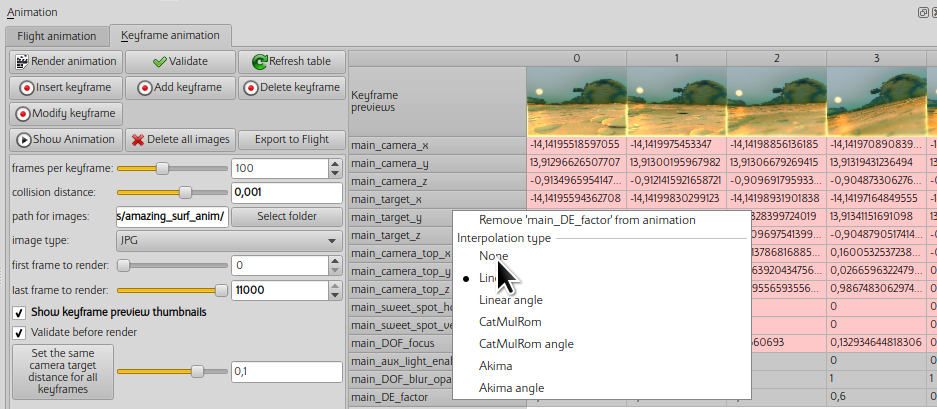
\includegraphics[width=6.69291in,height=2.92087in]{img/manual/media/image27.png}

\section{NetRender}\label{netrender}

NetRender is a tool that allows you to render the same image or
animation on multiple computers simultaneously. If you have multiple
computers connected to an Ethernet network, you can greatly increase
overall computing power.

One of the computers (server) manages the process of rendering. It sends
a requests to the connected computers (clients) and collects the results
of rendering. Other computers (clients) render different portions of the
image and send it to the server. There can be only one server (master)
but clients (slaves) can be any number. The more clients, the faster the
rendering will be.

The Server is also the computer which renders the combined image .

The total number of CPUs (cores) used is the sum of server's CPUs cores
+ all client's CPUs cores.

\begin{enumerate}
\def\labelenumi{\arabic{enumi}.}
\item ~
  \subsection{Starting NetRender}\label{starting-netrender}

  \begin{enumerate}
  \def\labelenumii{\alph{enumii}.}
  \item ~
    \subsubsection{Server configuration}\label{server-configuration}
  \end{enumerate}
\end{enumerate}

On the computer which will be used as the Server, Mode is set to
\emph{Server.}

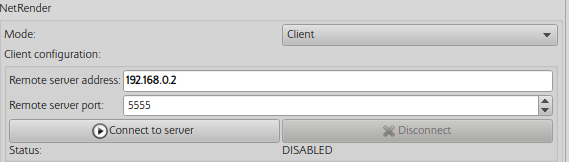
\includegraphics[width=4.53071in,height=1.86614in]{img/manual/media/image28.png}

\emph{Local server port} should be set to one which is not used by other
applications, and is passed through routers (if any are used) and
firewall. The default is 5555.

If settings are correct, press \emph{Launch server and watch for
clients} button to connect server to existing clients.

At this point, the server is ready to work

Alternative way to launch the server is to use command line. Example:

\$ mandelbulber2 -\/-server -\/-port 5555 pathToFileToRender.fract

\subsubsection{Configuring the clients}\label{configuring-the-clients}

On the computers which will be used as Clents, Mode is set to
\emph{Client}

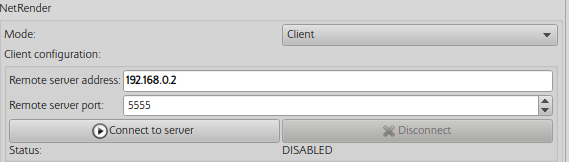
\includegraphics[width=5.02441in,height=1.43071in]{img/manual/media/image29.png}

The remote server address must be set to the same as the Server computer
which is running Mandelbulber in Server mode. The address can be given
as an IP address or a computer name.

The remote server port number must be exactly the same as the setting on
the Server.

Press \emph{Connect to server} button to connect to the server

Once the connection is established correctly, the client application
should show the status READY

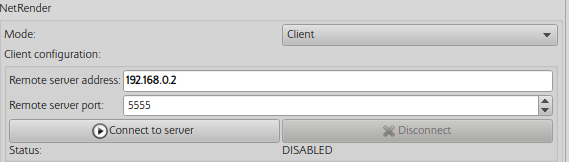
\includegraphics[width=5.07283in,height=1.48976in]{img/manual/media/image30.png}

Alternative way to establish NetRender client is to use command line:

\$ mandelbulber2 -\/-nogui -\/-host 10.0.0.4 -\/-port 5555

when connection is successfully established the program should return
following message:

NetRender - Client Setup, link to server: 10.0.0.4, port: 5555\\
NetRender - version matches (2090), connection
established\\[2\baselineskip]On the Server computer, in the table "List
of connected clients" should be shown the name and address of the
connected clients and the number of available processors (cores).

i.e magda computer has 4 cores and is READY.

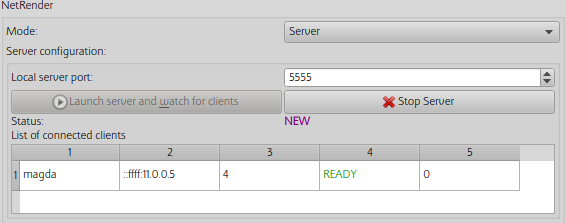
\includegraphics[width=5.07283in,height=1.99843in]{img/manual/media/image31.png}

\subsubsection{Rendering}\label{rendering}

Only the Server can initiate rendering on the computers connected using
NetRender. When the RENDER button is pressed on the server, all the
connected computers commence rendering.

In the table "List of connected clients'" in the column "Done lines"
will be shown the number of lines the image rendered by each of the
computers.

when rendering is finished, the Server computer, will display the
complete image. On the Client computers, only that portion of the image
which was rendered by that client will be displayed.

\section{Q\&A , Examples and Hints}\label{qa-examples-and-hints}

\textbf{Example of MandelboxMenger UI}

Example settings

(copy to clipboard, then load in Mandelbulber using : File -- Load
settings from clipboard):

\# Mandelbulber settings file

\# version 2.08

\# only modified parameters

{[}main\_parameters{]}

ambient\_occlusion\_enabled true;

camera 1.872135433718922 -2.023030528885091 1.871963531652841;

camera\_distance\_to\_target 0.005814178381115117;

camera\_rotation -28.76425655707408 26.3550335393397 3.450283685696816;

camera\_top -0.1604796308669786 -0.4174088010201082 0.894436236356597;

DE\_factor 0.6;

dont\_add\_c\_constant\_1 true;

flight\_last\_to\_render 0;

formula\_1 91;

formula\_2 61;

formula\_iterations\_2 5;

formula\_start\_iteration\_2 4;

formula\_stop\_iteration\_2 5;

fractal\_constant\_factor 0.9 0.9 0.9;

fractal\_enable\_2 false;

fractal\_rotation 0 -90 0;

keyframe\_last\_to\_render 0;

main\_light\_beta 44.34;

main\_light\_intensity 2;

mat1\_coloring\_palette\_offset 12.83;

mat1\_coloring\_palette\_size 255;

mat1\_surface\_color\_palette fd6029 698403 fff59c 000000 0b5e87 c68876
a51c64 3b9fee d4ffd4 aba53c;

SSAO\_random\_mode true;

target 1.874642452030676 -2.018463533070165 1.874544631933419;

view\_distance\_max 28.58330790625501;

volumetric\_fog\_colour\_1\_distance 3.55841069795292e-06;

volumetric\_fog\_colour\_2\_distance 7.116821395905841e-06;

volumetric\_fog\_distance\_factor 7.116821395905841e-06;

{[}fractal\_1{]}

fold\_color\_comp\_fold 0.3;

mandelbox\_color -0.27 0.05 0.07000000000000001;

mandelbox\_rotation\_main 9 1.74 3;

mandelbox\_scale -1.5;

transf\_addCpixel\_enabled\_false true;

transf\_int\_1 12;

transf\_scaleB\_1 0;

transf\_scaleC\_1 0;

transf\_start\_iterations\_M 4;

transf\_stop\_iterations\_M 5;\\[2\baselineskip]1) In the example the
MengerSponge part is run only on iteration 4. A single iteration of
another fractal to make a hybrid is often the best
practice.\\[2\baselineskip]2) In the Statistics (enable in View menu)
you can see Percentage of Wrong Distance Estimations ("Bad DE") is 0,
which is good!!. As a general rule less than 0.01 is good, but it is
case specific and 3.0 sometimes is OK and .0001 sometimes is not.

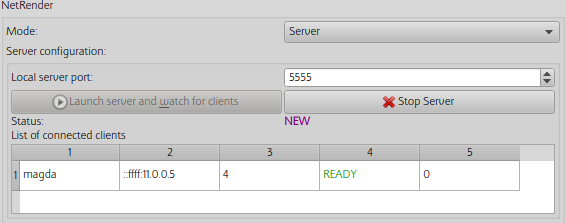
\includegraphics[width=4.51024in,height=2.48976in]{img/manual/media/image32.png}\\[2\baselineskip]T

The Raymarching step multiplier or "fudge factor" (Rendering Engine tab)
is set at 0.6, which is good for a hybrid. If I change it to 0.7 the
Percentage of Bad DE leaps up to 0.25 and you can see the areas of
quality loss on your image.\\[2\baselineskip]Now if we disable the
addCpixel Axis swap Constant Multiplier, we find we can now increase the
Raymarching Step Multiplier to 0.9, and get a faster render and visually
the same quality. So monitoring Percentage of Wrong Distance Estimations
is a guide to managing quality. ( Note when doing animations you may
want to drop the Raymarching step down a bit to allow for what might
happen between keyframes.)\\[2\baselineskip]3) MandelboxMenger Hybrids
can behave a bit differently to a lot of hybrids, in the fact that the
Percentage Bad DE often improves when you zoom in.

\textbf{maximum view distance}

Located : Rendering Engine - Common Rendering
settings\\[2\baselineskip]It is important to optimize this setting to
minimize render time. You can reduce until the furthest part of the 3D
object(s) starts to disappear. However with animation an allowance
should be made for changes between
keyframes.\\[2\baselineskip]hint/note.\\
When navigating in Relative step mode, mouse click on
spherical\_inversion, camera zooms out, tand maximum view distance
becomes set on 280. If you don't reset it your render times will be
increased.

\textbf{Magic Angle} Benesi Mag Transforms

In mathematics the Magic Angle = 54.7356° .

When rendering basic mag transforms the image does not render parallel
to the standard x,y,z global axis. On the fractal dock, in ``Global
parameters'' set y-axis rotation to 35.2644° ( = 90° - 54.7356°). The
fractal will then render parallel to the x-y plane.

\textbf{Example of using Transform\_Menger Fold to make
Hybrid}\\[2\baselineskip]\# Mandelbulber settings file

\# version 2.08

\# only modified parameters

{[}main\_parameters{]}

ambient\_occlusion\_enabled true;

camera -1.528388569045064 -1.23063017895654 -0.0251755516595821;

camera\_distance\_to\_target 0.0004503351519815117;

camera\_rotation -14.07789975269277 -44.28785609194563
3.773777260910995;

camera\_top 0.2333184436621841 0.6598138513697914 0.7142885869084139;

DE\_factor 0.7;

flight\_last\_to\_render 0;

formula\_1 1052;

formula\_2 1010;

formula\_3 1052;

formula\_4 1009;

formula\_iterations\_1 5;

formula\_start\_iteration\_4 45;

formula\_stop\_iteration\_2 12;

formula\_stop\_iteration\_4 5;

fractal\_constant\_factor 0.9 0.9 0.9;

fractal\_enable\_4 false;

hdr true;

hybrid\_fractal\_enable true;

keyframe\_last\_to\_render 0;

main\_light\_alpha 2.6;

main\_light\_beta 1.59;

mat1\_coloring\_palette\_offset 46.51;

mat1\_coloring\_palette\_size 255;

mat1\_coloring\_random\_seed 647723;

SSAO\_random\_mode true;

target -1.528310155903731 -1.230317492741513 -0.02549000429402527;

volumetric\_fog\_colour\_1\_distance 3.55841069795292e-06;

volumetric\_fog\_colour\_2\_distance 7.116821395905841e-06;

volumetric\_fog\_distance\_factor 7.116821395905841e-06;

{[}fractal\_1{]}

transf\_addition\_constantA\_000 -0.071633 0 0;

transf\_function\_enabledy false;

transf\_int\_1 12;

transf\_scale 0.5;

transf\_scaleC\_1 0;

transf\_stop\_iterations\_1 2;

{[}fractal\_2{]}

transf\_scale3D\_333 1.055556 1.027778 0.861111;

{[}fractal\_3{]}

transf\_function\_enabledx false;

On this transform UI, the standard menger sponge formula is split into a
start and end function. The simplest way to use this transform is in
Hybrid Mode, having the menger fold transform in slots 1 \& 3. In slot 2
place any linear type formula or transform. (ie more mengers, kifs,
mboxes, amazing surf, folds, rotation , Benesi T1
etc).\\[2\baselineskip]In slot 1 disable the stop function and in slot 3
disable the start function, resulting in a standard menger sponge with
something in the middle.\\[2\baselineskip]BTW in fact you can mix around
with the start and stop functions have all enabled if you wish.
Generally linear functions all work well together in making
hybrids.\\[2\baselineskip]In Statistics, maximum is approx. 80
iterations. Generally hybrids take longer to render than standard
formulas.\\[2\baselineskip]As well as adjusting formula parameters, you
can use the iteration controls to tweak hybrids. In this example the
first slot is set to repeat for 5 iterations before moving to slot 2.
Slot 2 is set to stop at iteration 12, whereas slots 1 \& 3 can continue
to termination conditions are met (bailout or maximum number of
iterations).

In the example above, slot2 of the hybrid sequenced ended at iteration
12. 12 was chosen because how it fitted into the iteration sequence, as
follows:\\[2\baselineskip]Slot1 x 5\\
0,1,2,3,4~ iteration numbers (note first iteration is iteration number
0.)\\[2\baselineskip]slot2\\
5\\[2\baselineskip]slot3~\\
6\\[2\baselineskip]slot1 x 5\\
7,8,9,10.11\\[2\baselineskip]slot2\\
12~ // last use of slot2\\[2\baselineskip]\hspace*{0.333em}sequence
continues slot1 x 5, slot3, .....to bailout.\\[2\baselineskip]So slot2
is used only twice in the iteration process. If I had entered 11 instead
of 12 for slot2's stop\_iterations, then the slot would have been used
only once, if I entered 19 then it would run three times.

\subsection{Q\&A . How do you get different materials on different
shapes?}\label{qa-.-how-do-you-get-different-materials-on-different-shapes}

This is how I have been doing it.\\[2\baselineskip]\emph{Rectangle at
the bottom marked A.}\\[2\baselineskip]This is where you~ start a new
material or load an existing.~ The active material is highlighted in
blue. Meaning it is active in the \textbf{material editor} where you
create or modify the material.\\[2\baselineskip]\emph{Rectangle at top
left marked B.}\\[2\baselineskip]One way to use a material is to go to
Global Parameters, click on the material preview image, and the
\textbf{Material Manager} UI will appear with the materials you have
loaded or created. Click on the one you want to use, then close that
UI.\\
Similarly with primitives, click on the material preview image. And with
Boolean Mode each fractal/transform has it's own material preview image
when you scroll down.

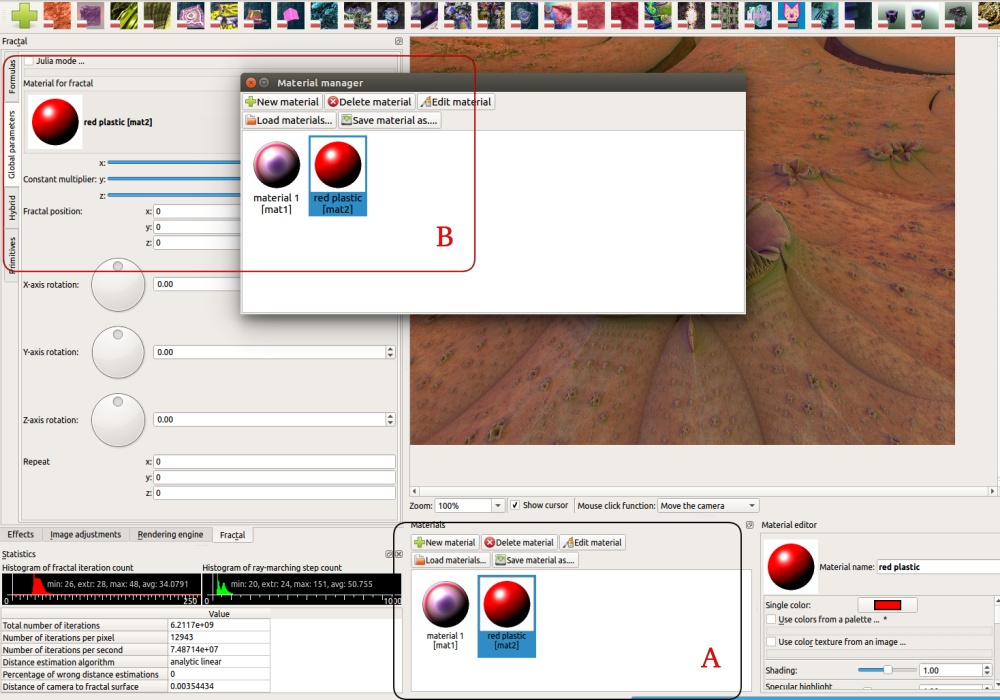
\includegraphics[width=6.69291in,height=4.68465in]{img/manual/media/image33.jpg}
